\section{Technische Grundlagen}
\subsection{Robotik} % Manuel ca. 8

\subsubsection{Grundlagen}
\subsubsection{Mobile Roboter}
\subsubsection{Antriebsarten}
\subsubsection{Sensorik}
\subsubsection{LEGO Mindstorm}

\newpage
\subsection{\gls{app} Entwicklung} %Simon ca. 8

\begin{wrapfigure}{r}{0.45\textwidth}
	\begin{center}
		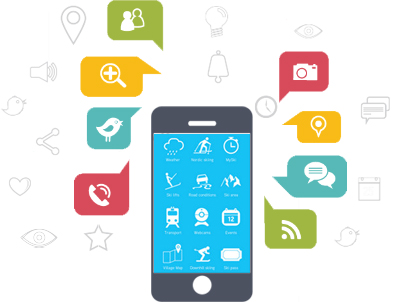
\includegraphics[width=0.4\textwidth]{images/technische_grundlagen/App-Development.jpg}
	\end{center}
	\caption{App Entwicklung}
	\label{fig:appentwicklung}
\end{wrapfigure}

Eine \gls{app} ist ein ausführbares Programm für mobile Geräte, wie Smartphones oder Tablets. Um eine App für ein mobiles Gerät zu entwickeln, müssen wie für andere Anwendungen im Voraus Anforderungen definiert werden, die die Anwendung erfüllen soll. Je nach festgelegten Anforderungen, die an das System gestellt werden, besteht eine begrenzte Anzahl von Möglichkeiten zur Verfügung. Allgemein kennt die \gls{app} Entwicklung drei verschiedene Arten, die native, web und hybride Entwicklung.

\subsubsection{Native \glspl{app}}

In der Entwicklung von nativen \glspl{app} werden die direkten Ressourcen des Gerätes verwendet. Dazu gehört die Laufzeitumgebung des Betriebssystemes, Bibliotheken und Hardwareschnittstellen. Der Vorteil von einer nativen Entwicklung liegt hauptsächlich darin, dass diese für das Betriebssystem optimiert ist und die vorhandenen Schnittstellen genutzt werden können, um komplexe und rechenintensive Anwendungen zu ermöglichen.\footnote{\citep[vgl.][Unterschiede und Vergleich native Apps vs. Web Apps]{DanielWurstl.Unterschiedeund}\label{note1}}\\
Vertreter diese Entwicklung finden sich für verschiedene Betriebssysteme. Der populärste unter ihnen ist bei weitem Android mit einer nativen Java Entwicklung über Android Studio von Google. Sie besitzt aktuellen den höchsten Marktanteil und eine entsprechende Popularität unter Entwickler und Nutzer.

\subsubsection{Web \glspl{app}}

Die Entwicklung von web \glspl{app} arbeitet mit systemübergreifenden Ressourcen und greift dabei auf gängige Webtechnologien, wie \gls{html}, \gls{css} und \gls{javascript} zurück. Die \gls{app} wird hierbei nicht wie normale Anwendungen direkt auf dem System des Gerätes ausgeführt, sondern kommt in dessen \gls{browser} zur Ausführung. Der Vorteil hierbei ist vor allem, dass diese Art von \gls{app} auf allen Betriebssystemen lauffähig ist und direkt über das Internet veröffentlicht und aktualisiert werden kann, jedoch wird eine stabile Internetverbindung vorausgesetzt.\footref{note1}\\
Von dieser Entwicklung finden sich viele Vertreter mit der Unterstützung diverser Frameworks. Das populärste unter ihnen ist aktuell AngularJS von Google, was auf \gls{javascript} basiert. In Kombination mit anderen Webtechnologien, wie gls{html} und \gls{css} lassen sich perfomante web \glspl{app} entwickeln.

\subsubsection{Hybride \glspl{app}}

Die Entwicklung von hybride \glspl{app} vereinigt die beiden Entwicklungen von native und web. Sie besteht dabei aus einem nativen Rahmen, in der eine web \gls{app} zur Ausführung kommt, diese besitzt entsprechende Zugriffsrechte auf Hardwareschnittstellen, um diese mit \glspl{api} anzusprechen.\footnote{\citep[vgl.][Native App, Web App und Hybrid App im Überblick]{PetraRiepe.NativeApp}\label{note2}}\\
Diese Entwicklung ist aktuell noch sehr jung, jedoch stechen hier bereits verschiedene Vertreter hervor. Der populärste unter ihnen ist Ionic von Drifty, was auf Apache Cordova als Basis zurückgreift. In Kombination mit AngularJS, TypeScript und anderen Webtechnologien lässt sich die web \gls{app} entwickeln und auf einem beliebigen Gerät unter einem nativen Browser ausführen. Es unterstützt dabei verschiedenste Betriebssystem, wie Android, iOS und Windows. Diese Entwicklungen können dabei meist nicht nur mobil, sondern unter anderem auf weiteren Systemen, wie stationäre bereitgestellt werden.

\subsubsection{Plattformübergreifende Programmierung}

\subsubsection*{Xamarin}
\subsubsection{Mono}
\subsubsection{.Net Framework}

\subsection{Java} %Gemeinsam ca. 2

\subsubsection{Grundlagen}
\subsubsection{Java Runtime Environment}

\subsection{Kommunikation} %Manuel ca. 5

\subsubsection{Grundlagen}
\subsubsection{TCP/IP}
\subsubsection{Wifi}
\subsubsection{Datenaustausch} %(JSON und Serialisierung)

\section{Theoretische Grundlagen}

\subsection{Schwarmverhalten}
\subsubsection{Allgemein}
\subsubsection{Vorbilder aus dem Tierreich}
% Fische, Bienen, Ameisen
\subsubsection{Szenarien}
\subsubsection{Algorithmen}